\documentclass[11pt]{article}

\usepackage[a4paper, margin=2.5cm]{geometry}
\usepackage{amsmath, amssymb}
\usepackage{booktabs}
\usepackage{graphicx}
\usepackage{caption}
\usepackage{setspace}
\usepackage[round]{natbib}
\usepackage{xcolor}
\definecolor{linkblue}{RGB}{28, 92, 171}
\usepackage[colorlinks=true, linkcolor=linkblue, citecolor=linkblue, urlcolor=linkblue]{hyperref}

\captionsetup{font=small, labelfont=bf}
\onehalfspacing

\title{\textbf{The S-Curve After the Shock:\\ Machine Learning Evidence on Mortgage Prepayment\\ in the Lock-In Era}}
\author{Luca Maffeis\thanks{This paper is a personal research project based exclusively on publicly
available data. The views expressed are the author's own and do not represent those of any employer.
Code and replication materials are available in the accompanying public repository. Not investment advice.}}
\date{July 2026}

\begin{document}

\maketitle

\begin{abstract}
\noindent
We estimate loan-level mortgage prepayment hazard models---logistic regression, gradient-boosted
trees, and a deep neural network in the spirit of \citet{sadhwani2021deep}---on 18.5 million Fannie
Mae loans observed monthly between 2018 and 2025, and use them to characterize how the prepayment
function changed after the 2022 interest-rate shock. A model estimated through 2021
over-predicted aggregate speeds by roughly 9 CPR at the onset of the shock, and its errors never
recovered: between 3.1 and 3.8 CPR points of cohort-level error in every year through 2025.
Annual re-estimation halved the error within a year, then needed about two more years of data to
get back below one point. The prepayment function itself did not flatten in the lock-in era, as
is sometimes argued; it rotated. Holding borrower composition fixed, the refinancing response
above the money is more than twice as steep as before the pandemic (30.5 versus 13.2 CPR at
$+150$ basis points of incentive), and the slow speeds of discount coupons are carried by the
level of prevailing rates rather than by a weaker incentive response. Applied to the December
2025 cross-section, the model places 2023--24 vintage 7.0\% coupons near 25 CPR at unchanged
rates and above 50 CPR in a 150 basis point rally. A caution for empirical work on this dataset:
several fields are blanked on removal records and can leak the prepayment event into standard
covariates, which---untreated---inflates out-of-sample AUC to 0.9999. All code and artifacts are
public.
\end{abstract}

\vspace{0.5em}
\noindent\textbf{Keywords:} mortgage prepayment; MBS; machine learning; lock-in effect;
gradient boosting; interpretability.

\section{Introduction}
\label{sec:intro}

Between March 2022 and October 2023 the 30-year fixed mortgage rate in the United States rose from
below 4\% to nearly 8\%, the fastest repricing of the mortgage market in four decades. Aggregate
conditional prepayment rates (CPR) on Fannie Mae collateral fell from above 35 to below 5, and by
the end of 2023 nearly the entire agency universe was out of the money. The episode placed
prepayment models---the central pricing input for a \$9 trillion market---outside the support of
their training data. The practitioner record of the aftermath is extensive: vendor models missed
monthly aggregate prints by 10--25\% through 2023--2025, disagreed on the sign of convexity below
par, and generated relative-value signals that inverted against realized returns
\citep{yu2023uncharted, katz2024models}.

A parallel academic literature has quantified the underlying mechanism---rate lock-in---from the
housing side. \citet{batzer2024lockin} estimate that each percentage point by which prevailing
rates exceed a borrower's contract rate reduces the probability of sale by 18.1\%;
\citet{fonseca2024lockin} find a 9--16\% reduction in moving probability per percentage point of
lock-in; \citet{liebersohn2025mobility} attribute a 16\% decline in the mobility of mortgaged
households to the mechanism. This literature measures the turnover component of prepayment, but
does not address the model-side question that concerns fixed-income practitioners: \emph{what
exactly changed in the prepayment function, and how should data-driven models be managed across
such a break?}

This paper provides one of the first public model-side treatments of the 2022 regime break
estimated on open data. We construct a monthly discrete-time hazard panel from the Fannie
Mae Single-Family Loan Performance dataset (18.5 million loans, 2018--2025), estimate three
classes of prepayment model of increasing flexibility under a strict walk-forward protocol, and
evaluate them at two levels: loan-level discrimination and---the economically relevant
metric---UPB-weighted cohort-level CPR error against full-population actuals.

The first set of results concerns model governance across the break
(Section~\ref{sec:e1}). The pre-shock model fails immediately, and its errors never
mean-revert: 3.1 to 3.8 CPR points of UPB-weighted cohort error in every year from 2022 through
2025. A structurally broken model, in other words, could not be ``ridden out.'' Re-estimation
worked, but slowly---annual refits improve steadily and still need roughly two years of
new-regime data before cohort errors fall below one CPR point, a pace of recovery that matches
what has been documented for commercial models over 2023--25.

The second set of results concerns the shape of the prepayment function
(Section~\ref{sec:e2}). Estimating the model separately by regime and tracing each fit's
partial-dependence S-curve on a fixed reference population separates composition from behavior,
and the answer is not the flattening that is sometimes claimed. Conditional on composition, the
refinancing limb of the lock-in-era S-curve is \emph{steeper} than its pre-pandemic
counterpart: the elasticity through the cusp rises from 2.2 to 12.6 CPR points per 100 basis
points. Depressed deep-discount turnover, meanwhile, is absorbed by the prevailing-rate level
rather than by a decayed incentive response. Both sides of a live practitioner debate
\citep{sancap2024scurves, katz2024models} turn out to be describing the same estimated function.

Finally, the estimates translate into a forward-looking statement about the current coupon
stack (Section~\ref{sec:e3}). As of December 2025, model-implied speeds for the 2023--24
vintage 6.5--7.0\% coupons rise steeply under modest rallies; the 6.5s roughly triple between
unchanged rates and a 150 basis point rally.

A secondary, methodological contribution concerns data quality. Three fields in the public
dataset are blanked on a loan's terminal record, so that---if used contemporaneously---their
missingness perfectly reveals the prepayment event. Untreated, these produce out-of-sample AUCs
of 0.9999 and would invalidate any study built on them. Section~\ref{sec:leakage} documents the
mechanism and the corrections, which we regression-test in the released code.

\section{Related literature}
\label{sec:lit}

\paragraph{Machine learning for mortgage risk.} \citet{sadhwani2021deep} estimate multi-state
transition models on 120 million U.S. mortgages with deep neural networks and document large
out-of-sample gains over logistic benchmarks, with prepayment exhibiting the strongest
nonlinearities. \citet{zhang2019agency} deploy neural networks for agency MBS prepayment at pool
level and interpret the fitted model through implied S-curves, burnout, and seasonality;
\citet{schultz2021rise} make the case for gradient-boosted trees at loan level.
\citet{blumenstock2022deep} find machine-learning survival models dominate statistical benchmarks
for competing default and prepayment risks; \citet{ojha2021comparing} compare conventional and
deep learners on Fannie Mae data through the financial crisis. Relative to this literature, our
contribution is not architectural novelty but the regime question: all published samples of which
we are aware end before or shortly after the 2022 break, and none addresses model management
across it.

\paragraph{The lock-in effect.} \citet{batzer2024lockin}, \citet{fonseca2024lockin}, and
\citet{liebersohn2025mobility} establish the magnitude of rate lock-in for housing turnover,
labor mobility, and welfare. We use their elasticities as external anchors for the
turnover-suppression channel recovered by our models.

\paragraph{Practitioner record.} \citet{yu2023uncharted} frames post-2022 prepayment modeling as
an out-of-sample problem; monthly commentary by Santander US Capital Markets documents production
model errors of 10--25\% through 2023--25 and argues that apparent S-curve flattening reflects
spread-at-origination (SATO) composition \citep{sancap2024scurves}; \citet{katz2024models} document
model-implied relative value inverting against realized returns in 2024 and, in early 2026,
pool-level S-curves exceeding pandemic-era steepness. Our per-regime, composition-controlled
S-curves reconcile these observations within a single estimated model.

\section{Data}
\label{sec:data}

\subsection{Loan-level performance data}

We use the Fannie Mae Single-Family Loan Performance dataset, acquisition quarters 2018Q1 through
2025Q4: 18,468,917 fixed-rate loans and their complete monthly servicing records through December
2025, parsed from the raw 113-field pipe-delimited files. The window brackets three regimes:
pre-pandemic (2018--19), the pandemic refinancing wave (2020--21), and the lock-in era
(2022--25). Voluntary prepayment is identified by zero-balance code 01 (payoff); credit events
and repurchases are treated as censoring.

\subsection{Cohort-level ground truth}

From the full population---prior to any sampling---we compute actual cohort-level single monthly
mortality and CPR by vintage year and coupon (rounded to the nearest 0.5), where SMM is
voluntarily prepaid UPB over beginning-of-month UPB. These series serve as the evaluation target
for all models and align with public anchors: 2023-vintage 7.0 coupons print 5.4 CPR in June
2024, peak at 30.3 in the October 2024 refinancing episode, and revert to 9.1 by December
\citep{fhfa2024pmr}; 2021-vintage 2.5 coupons remain at 2--4 CPR throughout 2023--25; 2018-vintage
4.5 coupons run at 41--57 CPR through the pandemic wave \citep{haughwout2023refi}.

\subsection{Estimation panel}

A deterministic, hash-based stratified sample (vintage year $\times$ note-rate bucket, with
inverse-probability loan weights) of 1,201,243 loans yields a monthly hazard panel of 2,532,987
loan-month observations containing all 428,793 voluntary prepayment events and a 5\%
importance-weighted subsample of non-event months. Weights are carried through estimation and
aggregation, so fitted hazards are on the monthly SMM scale and cohort aggregates are
population-representative.

Covariates comprise: the refinancing incentive (note rate minus the Freddie Mac PMMS 30-year
survey rate); spread at origination (SATO); burnout (cumulative positive incentive over prior
months); mark-to-market LTV (original LTV revalued with state-level FHFA house-price indices);
loan age; original balance; credit score; DTI; original LTV; calendar month; the prevailing
mortgage-rate level; and categorical origination attributes (channel, purpose, property type,
occupancy, state, borrower count, first-time-buyer flag) plus lagged delinquency status and
modification flag.

\subsection{Removal-record measurement pitfalls}
\label{sec:leakage}

Three covariates initially produced out-of-sample AUCs of 0.9999---a value that should be read as
diagnostic of leakage rather than of predictive skill. The mechanism is systematic: the dataset
blanks monthly-reported fields on a loan's terminal record. Consequently (i) mark-to-market LTV
computed on the end-of-period balance equals exactly zero if and only if the loan prepaid that
month; (ii) the modification flag and delinquency status are missing on removal records, so their
missingness indicators reveal the event; and (iii) the reported loan-age field is likewise
blanked. All state-dependent inputs are therefore measured as of the \emph{beginning} of the
month---balances lagged (the factor-date convention), status fields lagged one month, and loan age
computed from calendar arithmetic rather than read from the file. Each correction carries a
regression test in the released code. Post-correction discrimination falls to the 0.59--0.75
range, which we regard as the honest difficulty of monthly voluntary-prepayment classification.

\section{Methodology}
\label{sec:method}

\subsection{Hazard framework and inverse-probability weighting}
\label{sec:ipw}

Let $y_{it} \in \{0,1\}$ indicate voluntary prepayment of loan $i$ in month $t$. We model the
discrete-time hazard $h_{it} = \Pr(y_{it}=1 \mid x_{it})$, where $x_{it}$ contains only
information available at the beginning of month $t$.

The estimation panel is drawn from the population in two independent, deterministic stages, and
every observation carries the inverse of its inclusion probability. Stage one samples
\emph{loans}: within stratum $s(i)$ (vintage year $\times$ note-rate bucket), loan $i$ is
included with probability $\pi_{s(i)} = \min\{1,\, \bar n / N_{s(i)}\}$, where $N_s$ is the
stratum size and $\bar n$ the per-stratum target, implemented by a hash of the loan identifier
(no random-number generator, hence exactly replicable). Stage two samples \emph{loan-months}:
every event month ($y_{it}=1$) of a sampled loan is retained with probability one, while
non-event months are retained with probability $\kappa = 0.05$, again by hashing. The combined
design weight is therefore
\begin{equation}
w_{it} \;=\;
\begin{cases}
1/\pi_{s(i)}, & y_{it}=1,\\[2pt]
1/\bigl(\pi_{s(i)}\,\kappa\bigr), & y_{it}=0 .
\end{cases}
\end{equation}
For any population functional expressible as a sum over loan-months,
$S = \sum_{it} z_{it}$, the weighted sample sum $\hat S = \sum_{it \in \mathcal{S}} w_{it}
z_{it}$ is a Horvitz--Thompson estimator and is unbiased, since each term's inclusion
probability is exactly $\pi_{s(i)}$ or $\pi_{s(i)}\kappa$ by construction. Two consequences
follow. First, maximizing the $w$-weighted log-likelihood targets the population likelihood, so
fitted hazards are calibrated to the population base rate---retaining all events while
down-sampling non-events does \emph{not} require the usual post-hoc intercept correction for
case-control sampling, because the weights already undo the design. Second, population
cohort-level speeds are recovered by weighting fitted hazards with the product of design weight
and beginning-of-month balance $b_{it}$: for cohort $c$ in month $t$,
\begin{equation}
\widehat{\mathrm{SMM}}_{ct} \;=\; \frac{\sum_{i \in c} w_{it}\, b_{it}\, \hat h_{it}}
{\sum_{i \in c} w_{it}\, b_{it}}, \qquad
\widehat{\mathrm{CPR}}_{ct} \;=\; 1 - \bigl(1 - \widehat{\mathrm{SMM}}_{ct}\bigr)^{12},
\end{equation}
where numerator and denominator are each Horvitz--Thompson estimators of their population
counterparts (expected voluntarily-prepaid balance and total beginning balance). Evaluation
never relies on the sampled denominator where the population value is available: actual cohort
CPRs are computed on the \emph{full} population of Section~3.2. Appendix~\ref{app:robustness}
verifies empirically that results are insensitive to halving $\kappa$, and that fitted hazards
are well calibrated against weighted empirical event rates.

\subsection{Estimators}

We estimate three models of increasing flexibility on identical features and weights: (i)
weighted logistic regression (median-imputed numerics, one-hot categoricals)---the linear
benchmark; (ii) gradient-boosted trees (LightGBM; 63 leaves, 600 trees, learning rate 0.05,
minimum 100 observations per leaf), with missing values handled natively; and (iii) a
feed-forward neural network with categorical embeddings (three hidden layers, 128--128--64 ReLU
units, dropout 0.1), trained with weighted cross-entropy, following the architecture spirit of
\citet{sadhwani2021deep}. We deliberately avoid early stopping on trailing-window validation sets:
in the presence of regime shifts, a trailing window is unrepresentative of both past and future,
and we found it induces severe underfitting precisely at the breaks.

\subsection{Evaluation protocol}

All evaluation is strictly walk-forward: models are estimated on months up to December of year
$T$ and evaluated on the following twelve months, for $T = 2018, \dots, 2024$. We report
loan-level weighted AUC, and UPB-weighted mean absolute cohort CPR error (in CPR points) against
the full-population actuals of Section~3.2. We emphasize the latter: loan-level discrimination
metrics have limited economic meaning for portfolio speeds, and---as Section~\ref{sec:leakage}
illustrates---are also the metrics most easily corrupted by leakage.

\section{Results}
\label{sec:results}

\subsection{Walk-forward performance}

Table~\ref{tab:walkforward} reports the walk-forward record. The gradient-boosted model beats
the logistic benchmark on cohort-level error in six of seven windows, and the gap is widest
exactly where it matters for the questions of this paper: 0.9 versus 6.1 CPR points at the 2024
split. Neither model gets the \emph{level} of the 2020--21 refinancing wave right. Commercial
models did not either; the determinants of wave amplitude (origination capacity, appraisal
waivers, media effects) are simply not spanned by loan-level covariates, and we flag this
honestly rather than tune it away. It is also worth dwelling on the AUC column: discrimination
deteriorates for every model in the lock-in era. With the entire universe out of the money, who
prepays in a given month is close to idiosyncratic, so a low lock-in-era AUC is a property of
the environment, not a defect of any particular learner. As for the neural network, evaluated
at three splits it is competitive on discrimination (AUC 0.75/0.65/0.64) and ahead of the trees
on cohort error at the pre-wave split (8.8 versus 12.2 CPR points), but it falls behind in the
lock-in era (4.6 versus 3.7, and 1.5 versus 0.9) and under-predicts the hazard level. At 2.5
million training rows a mixed result is what the tabular-learning literature would predict;
the deep-learning advantage in \citet{sadhwani2021deep} was demonstrated on three orders of
magnitude more data. The gradient-boosted model is therefore the engine for the experiments
that follow.

\begin{table}[ht]
\centering
\small
\begin{tabular}{lcccc}
\toprule
Training window ends & \multicolumn{2}{c}{Loan-level AUC} & \multicolumn{2}{c}{Cohort CPR MAE (pts)} \\
\cmidrule(lr){2-3}\cmidrule(lr){4-5}
 & Logistic & GBM & Logistic & GBM \\
\midrule
2018-12 & 0.66 & 0.71 & 11.6 & 6.4 \\
2019-12 & 0.75 & 0.78 & 12.7 & 12.2 \\
2020-12 & 0.72 & 0.75 & 8.6 & 13.1 \\
2021-12 & 0.61 & 0.66 & 4.6 & 3.7 \\
2022-12 & 0.52 & 0.63 & 2.6 & 2.2 \\
2023-12 & 0.57 & 0.66 & 5.2 & 0.9 \\
2024-12 & 0.59 & 0.69 & 6.1 & 0.9 \\
\bottomrule
\end{tabular}
\caption{Walk-forward evaluation. Each row: estimation through December of the stated year,
evaluation on the subsequent twelve months. Cohort CPR MAE is UPB-weighted across vintage
$\times$ coupon cohorts against full-population actuals. The 2020--12 test window is the peak of
the pandemic refinancing wave.}
\label{tab:walkforward}
\end{table}

\subsection{The regime break: error persistence and the pace of recovery}
\label{sec:e1}

We compare a model frozen at December 2021 against annual re-estimation, both walked forward over
2022--25 (Figure~\ref{fig:e1}). The onset is brutal: in January 2022 the frozen model predicts
aggregate speeds of approximately 19 CPR against an actual print of 11, an error of nearly 9
CPR points, because it extrapolates refinancing-wave behavior into a market that has just
repriced. Over 2022 as a whole its UPB-weighted cohort error is 3.7 CPR points. What the
aggregate figures cannot show, and the annual errors can, is that the frozen model never gets
better: 3.8 points in 2023, 3.3 in 2024, 3.1 in 2025. The errors do not decay as the lock-in
era matures, because the model's learned response surface---not merely its level---is wrong for
the new regime; Figure~\ref{fig:e1} shows it running 2--4 points above realized speeds in
essentially every month after mid-2022. Re-estimation recovers, but on data's schedule rather
than management's: folding in the 2022 transition year nearly halves the 2023 error (2.2 versus
3.8 points), and with two full years of post-break observations the annually re-estimated model
reaches 0.9 points in both 2024 and 2025, comparable to pre-break accuracy. The governance
lesson cuts both ways. A structurally broken model cannot be ridden out in the hope that its
errors mean-revert, and recalibration works but only at the pace at which new-regime
observations accumulate. Both halves are consistent with the documented difficulties of commercial models over
2023--25 \citep{yu2023uncharted, katz2024models}.

\begin{figure}[ht]
\centering
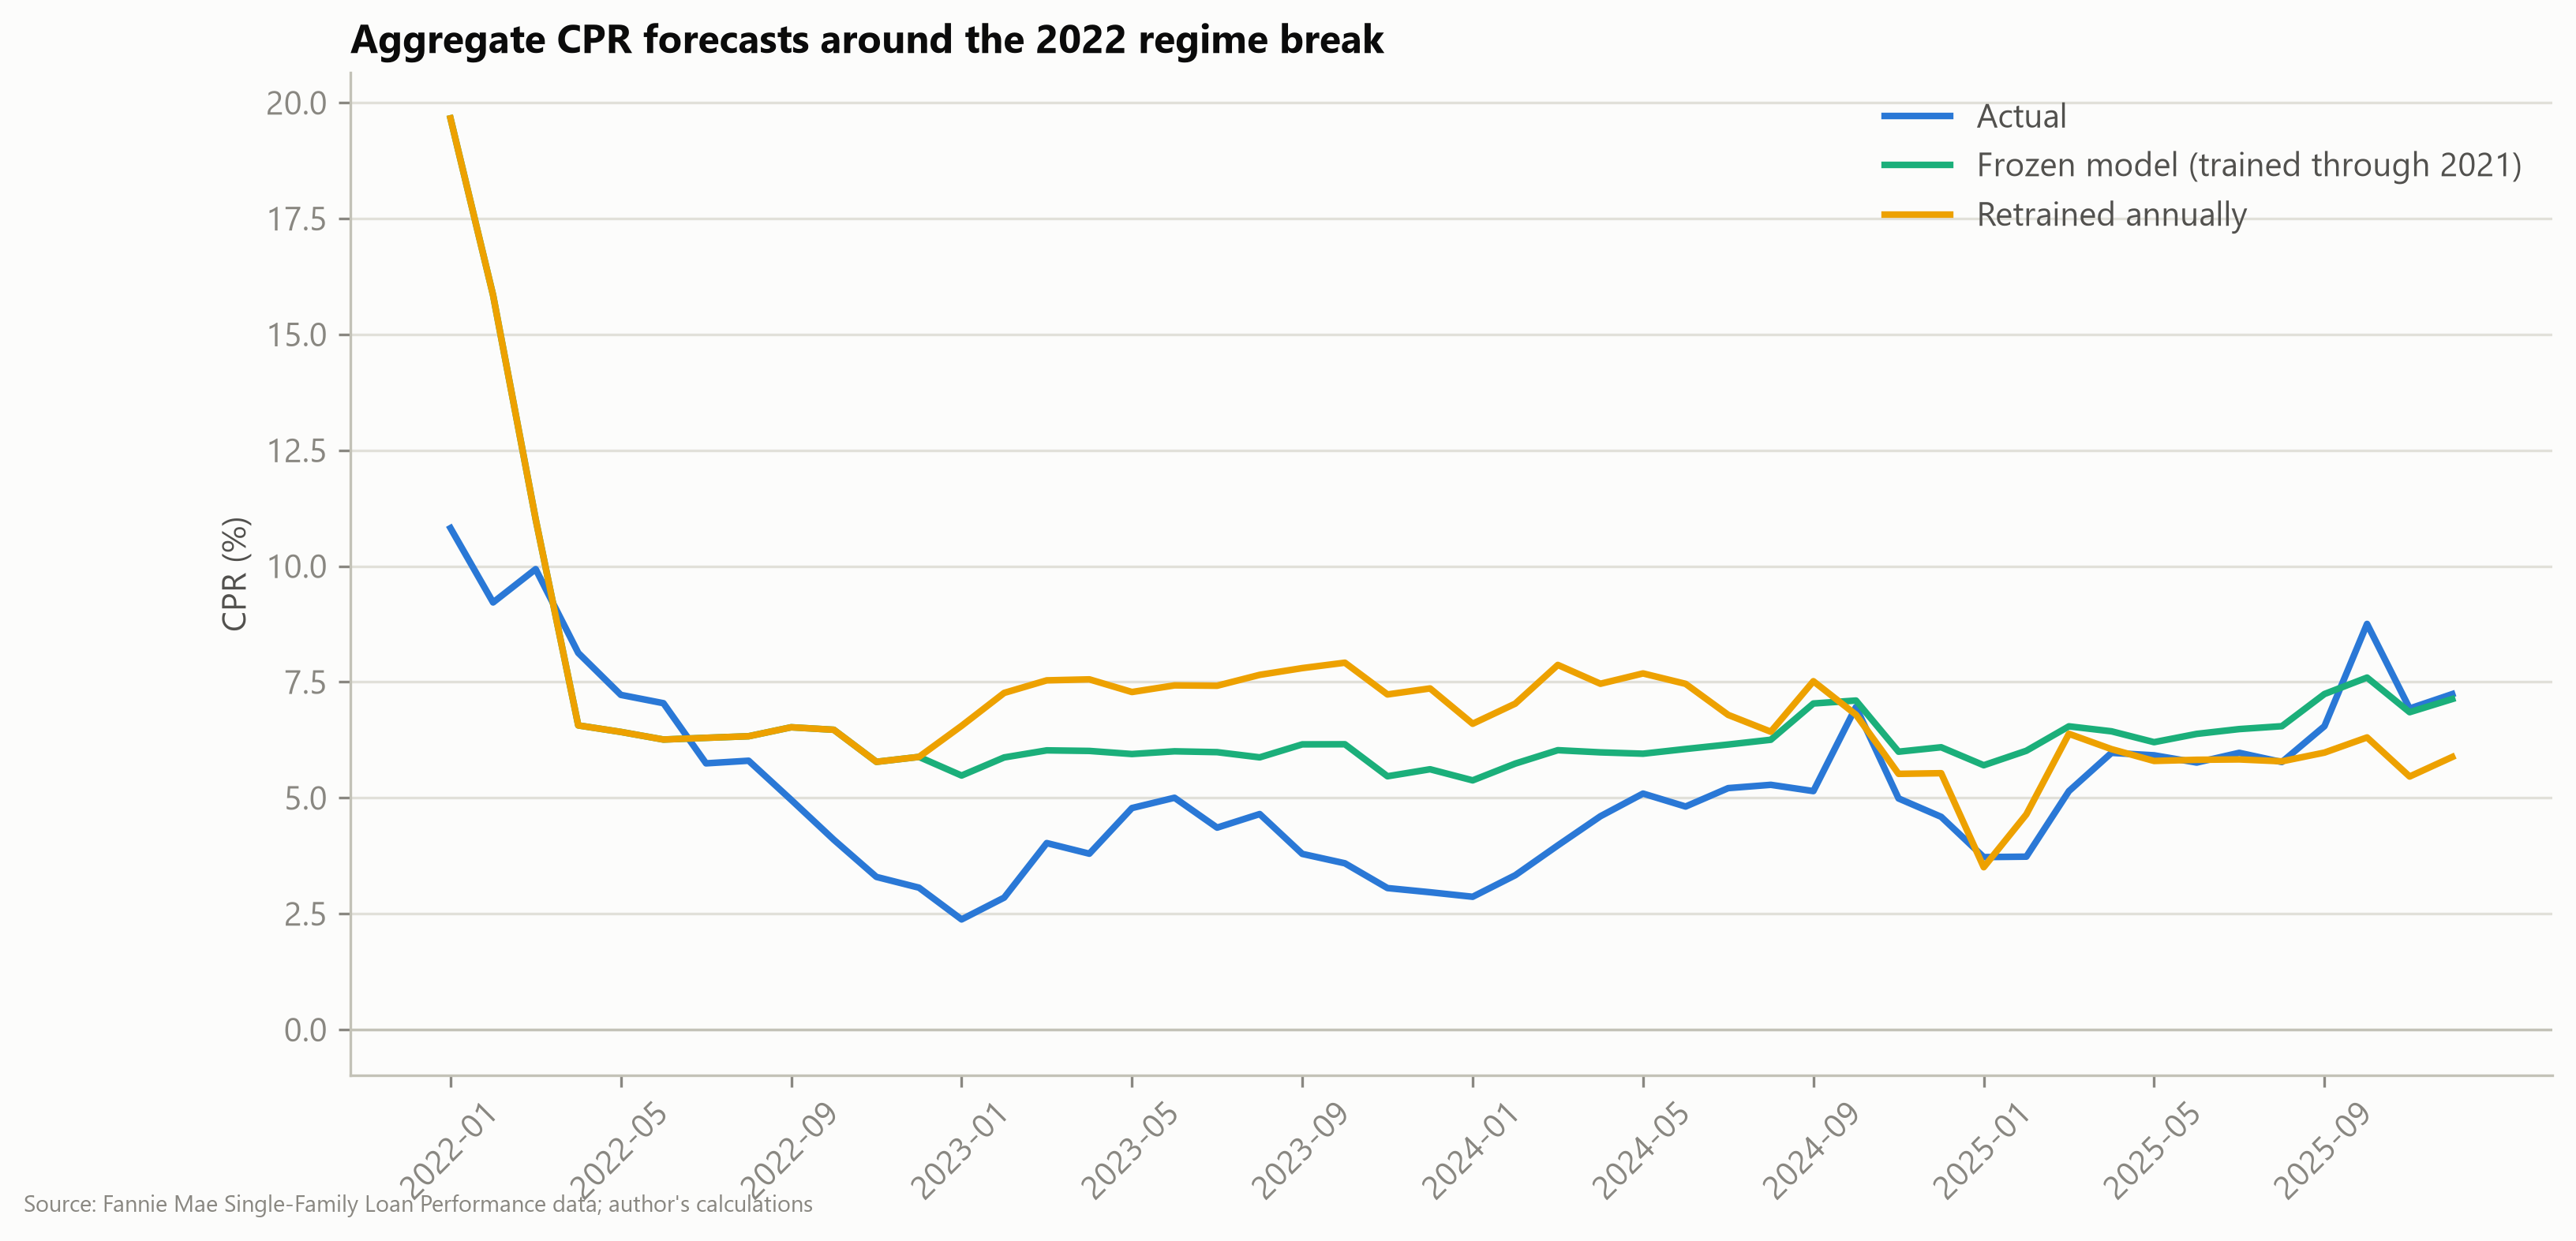
\includegraphics[width=0.95\textwidth]{figures/e1_frozen_vs_retrained.png}
\caption{Aggregate UPB-weighted CPR, 2022--2025: actuals versus a model frozen at December 2021
and a model re-estimated each year-end. The two model series coincide during 2022 by
construction. The frozen model over-predicts by $\approx 9$ CPR points at the January 2022 onset
and remains 2--4 points above realized speeds through 2025; the re-estimated model converges to
realized speeds from 2024 onward.}
\label{fig:e1}
\end{figure}

\subsection{The learned S-curve, by regime}
\label{sec:e2}

We estimate the gradient-boosted model separately on each regime---pre-pandemic (2018-01 to
2019-12), refinancing wave (2020-04 to 2021-12), and lock-in (2022-07 to 2025-12)---and trace
each fitted model's partial-dependence function of the refinancing incentive on a \emph{common}
reference population of 200,000 lock-in-era loan-months. Holding the population fixed ensures
that differences between curves reflect learned behavior rather than composition.
Figure~\ref{fig:e2} and Table~\ref{tab:e2} report the results.

\begin{figure}[ht]
\centering
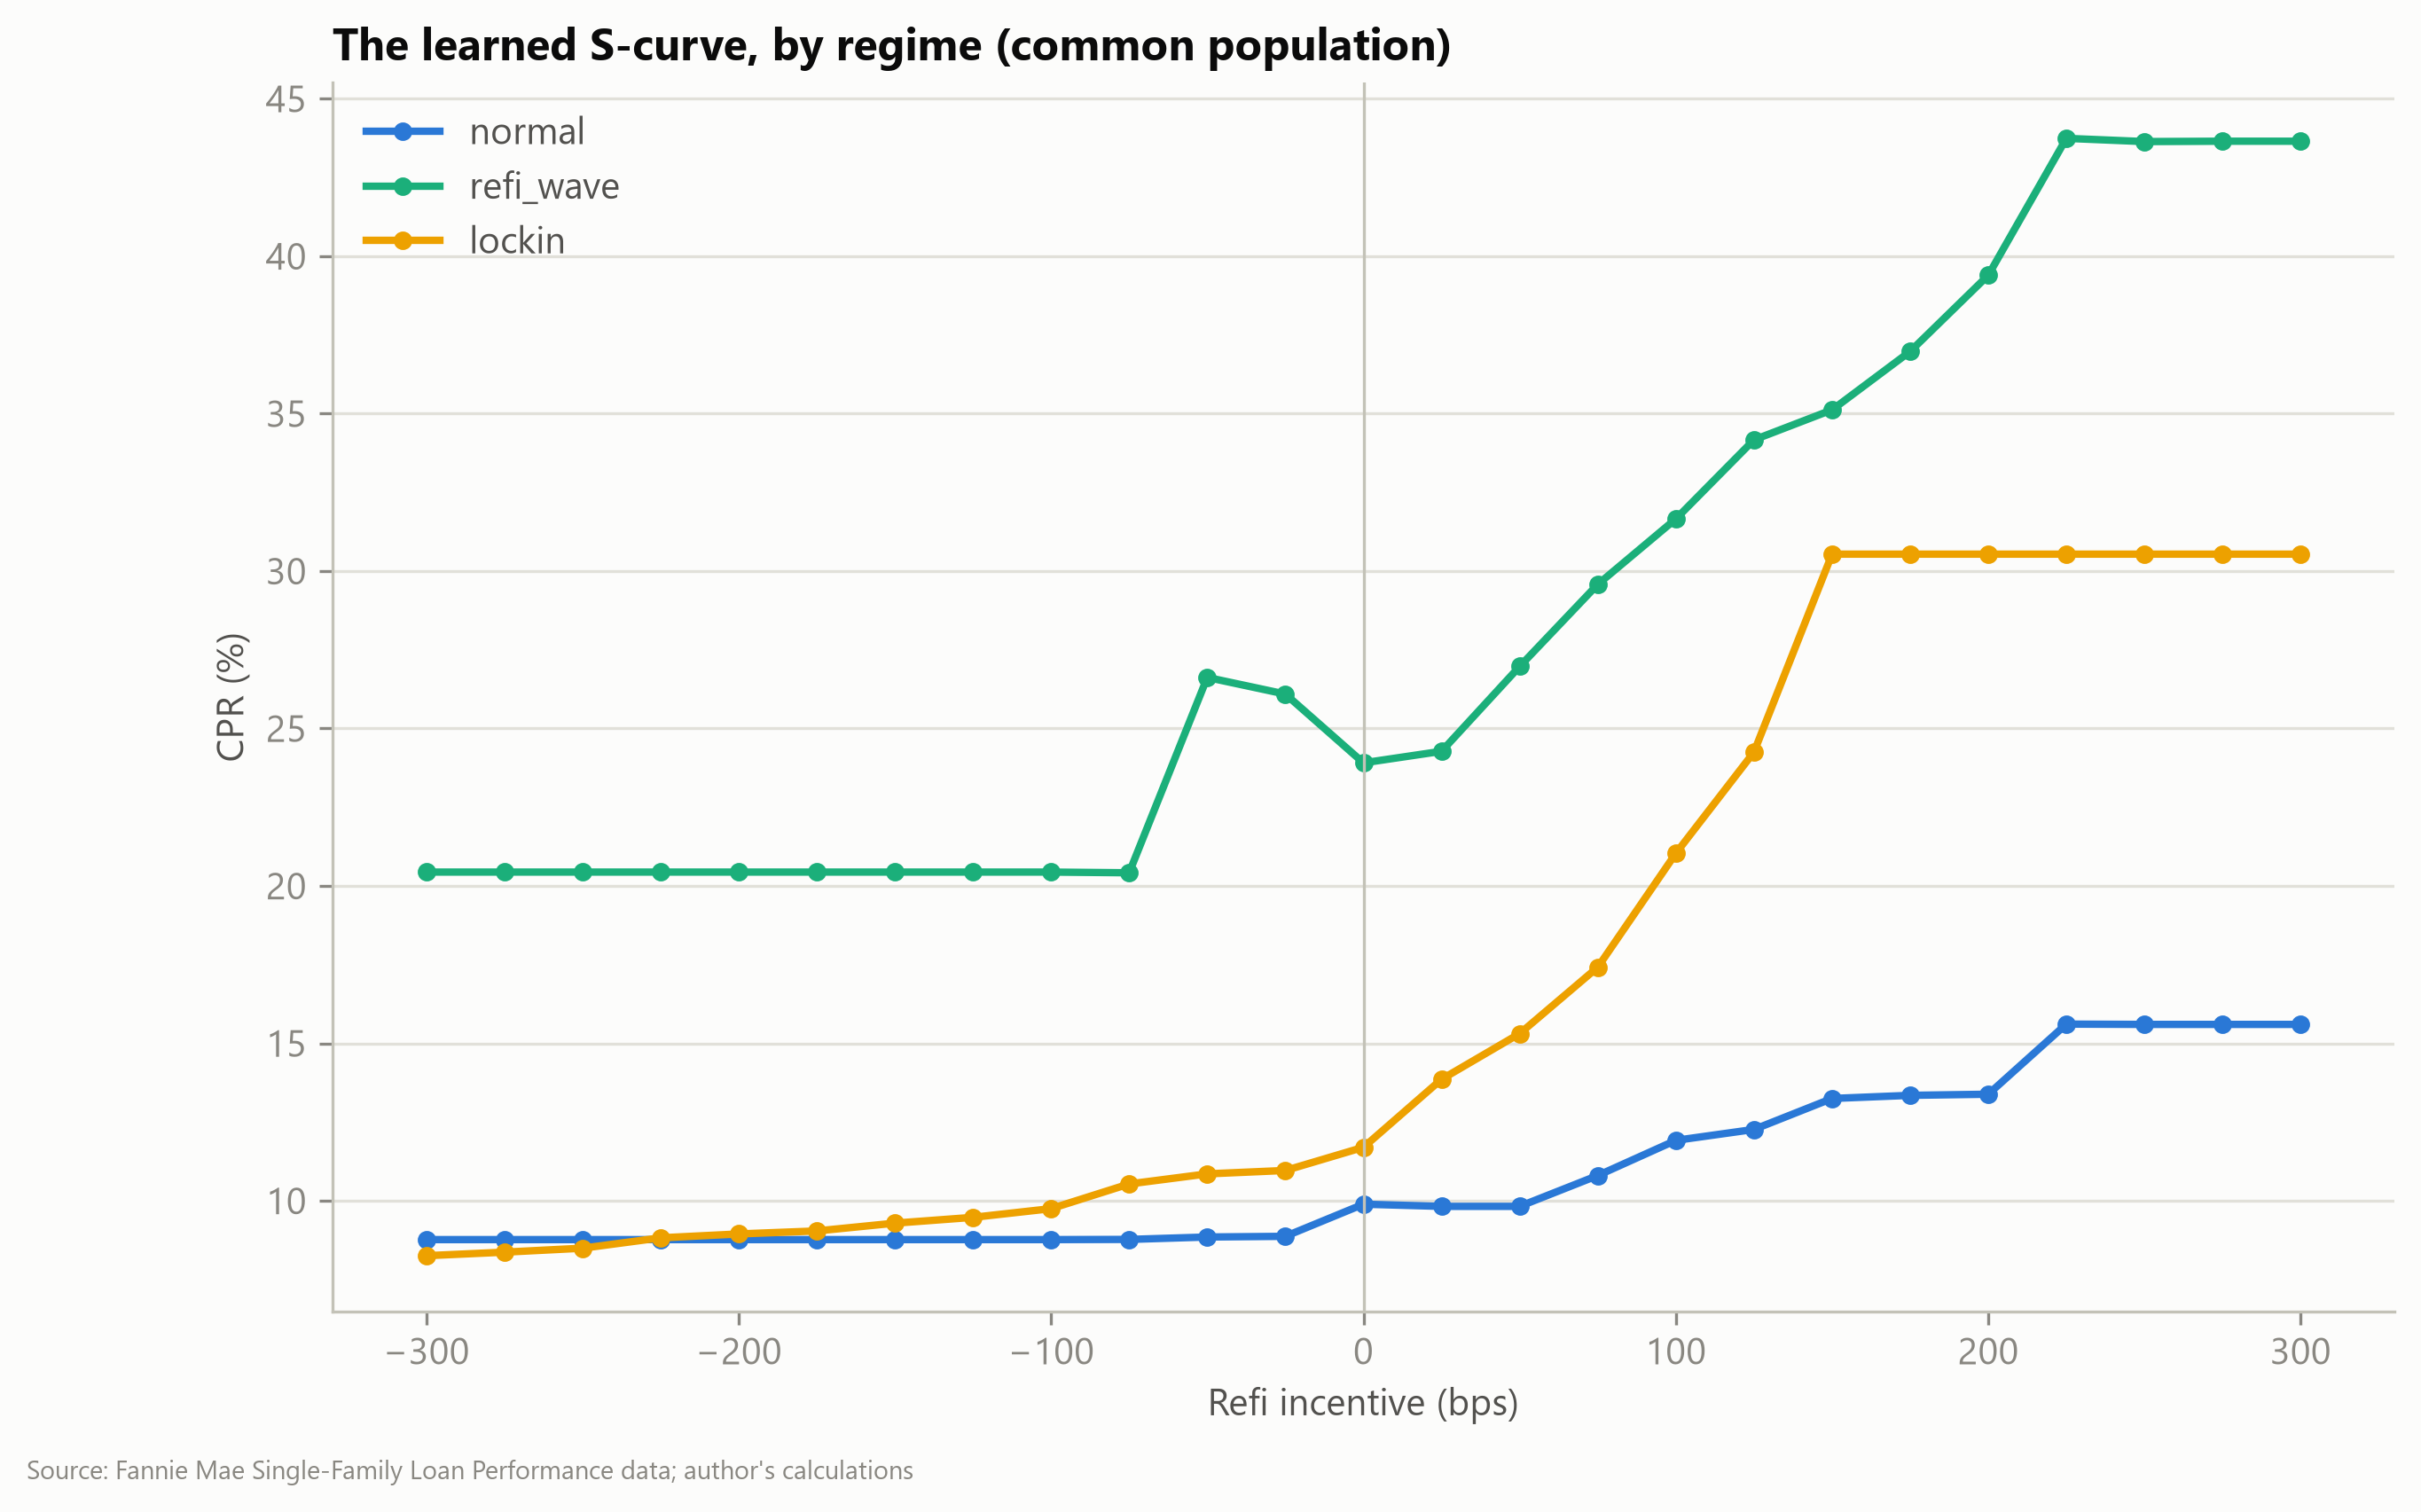
\includegraphics[width=0.82\textwidth]{figures/e2_scurves.png}
\caption{Model-implied S-curves (partial dependence of annualized speed on refinancing
incentive) by estimation regime, evaluated on a common lock-in-era reference population.}
\label{fig:e2}
\end{figure}

\begin{table}[ht]
\centering
\small
\begin{tabular}{lcccc}
\toprule
Regime & CPR at $-200$bp & CPR at $0$ & CPR at $+150$bp & Elasticity (pts/100bp) \\
\midrule
Pre-pandemic 2018--19 & 8.8 & 9.9 & 13.2 & 2.2 \\
Refinancing wave 2020--21 & 20.4 & 23.9 & 35.1 & 7.5 \\
Lock-in 2022--25 & 8.9 & 11.7 & 30.5 & 12.6 \\
\bottomrule
\end{tabular}
\caption{S-curve landmarks by regime on the common reference population. Elasticity is the
average slope between 0 and $+150$ basis points of incentive. All entries are
partial-dependence values: counterfactual model responses obtained by setting the incentive to
the stated level for every observation in the fixed reference population. They are not realized
cohort speeds and should not be compared directly to observed cohort CPRs (see text).}
\label{tab:e2}
\end{table}

The central finding is a rotation, not a flattening. The refinancing limb of the lock-in-era
S-curve is markedly steeper than its pre-pandemic counterpart: 30.5 versus 13.2 CPR at $+150$
basis points, an elasticity through the cusp of 12.6 versus 2.2 CPR points per 100 basis points.
Borrowers who reach the money in the lock-in era refinance faster than any pre-2020 cohort
would have---consistent with the 15-month average age at refinancing observed in the 2024
episode and with the efficiency of modern origination channels. At the deep-discount end, the
lock-in model's implied turnover on the common population is close to pre-pandemic levels; the
observed 2--4 CPR prints of deeply out-of-the-money cohorts are reproduced through the
prevailing-rate-level covariate---the lock-in channel of \citet{batzer2024lockin}---rather than
through a degraded incentive response.

A word on how to read (and how not to read) Table~\ref{tab:e2}. Partial-dependence values at a
given incentive are averages over the \emph{entire} reference population with only the incentive
altered; every other covariate, including burnout, mark-to-market LTV, and the prevailing-rate
level, keeps its observed value. The population composition at, say, $-200$ basis points in the
table never occurs in any realized cohort. In particular, the tabulated 8.9 CPR for the lock-in
model at $-200$ basis points is not comparable to the 2--4 CPR prints of 2021-vintage 2.5\%
coupons: those cohorts sit at $-300$ to $-450$ basis points of incentive, at or beyond the left
edge of the evaluated grid where the curves are lower, and their suppressed turnover loads on
the rate-level covariate rather than on the incentive itself. And because the reference
population is held fixed across regimes, \emph{differences} between curves identify differences
in the learned response functions, while \emph{levels} inherit the reference population's
covariate mix and should be read only relative to one another. SATO-conditioned partial dependence (replication
materials) confirms the composition mechanism of \citet{sancap2024scurves}: within every regime,
higher-SATO tertiles trace steeper curves. The decomposition thus reconciles the composition
view with the observation of \citet{katz2024models} that late-2025 realized S-curves exceed
pandemic-era steepness: both are features of the same estimated function.

Attribution analysis (mean absolute SHAP values; replication materials) tells the same story at
the level of drivers: pre-pandemic prepayment is dominated by burnout and seasoning; the wave by
the incentive; and in the lock-in era all drivers compress, consistent with the decline in
achievable discrimination.

\subsection{Scenario read-through for the current coupon stack}
\label{sec:e3}

Finally, we apply the full-sample model to the December 2025 cross-section of active 2023--24
vintage 6.0--7.0\% coupons under parallel shifts of the mortgage rate, holding burnout and
house prices fixed (a deliberately transparent one-month-hazard exercise, annualized).
Table~\ref{tab:e3} reports projected speeds.

\begin{table}[ht]
\centering
\small
\begin{tabular}{lcccc}
\toprule
Cohort & Unchanged & $-50$bp & $-100$bp & $-150$bp \\
\midrule
2023 6.0s & 6.9 & 12.9 & 20.7 & 25.9 \\
2023 6.5s & 13.1 & 22.5 & 29.1 & 36.0 \\
2023 7.0s & 25.4 & 34.4 & 43.7 & 52.0 \\
2024 6.0s & 6.5 & 12.1 & 19.4 & 26.1 \\
2024 6.5s & 13.3 & 23.0 & 32.4 & 42.1 \\
2024 7.0s & 25.5 & 35.5 & 43.7 & 52.2 \\
\bottomrule
\end{tabular}
\caption{Model-projected CPR for the December 2025 cross-section of 2023--24 vintage cohorts
under parallel mortgage-rate shifts.}
\label{tab:e3}
\end{table}

The 7.0\% coupons are already fast at unchanged rates ($\approx$25 CPR) and reach
refinancing-wave speeds (above 50 CPR) under a 150 basis point rally; the 6.5s approximately
triple over the same interval and constitute the cuspiest segment. This is the model-implied
counterpart of the record negative convexity measured in the current-coupon market in late 2025
\citep{katz2024models}, localized to specific vintage-coupon cohorts.

\section{Limitations}
\label{sec:limitations}

Our sample is Fannie Mae collateral only; Ginnie Mae collateral---whose VA segment exhibited the
fastest and most policy-sensitive speeds of the 2024--25 episodes---is outside the dataset.
The pre-pandemic regime is observed for only two years (vintages 2018+). The scenario analysis
is a one-month hazard annualized with burnout and house prices held fixed; it understates path
dependence in a sustained rally and is not a valuation (OAS) model. The level of the 2020--21
wave is under-predicted by all specifications, ours and commercial alike, reflecting absent
capacity and media-effect covariates. Partial-dependence curves are counterfactuals on a fixed
population, not cohort forecasts. Finally, monthly PMMS timing and the publication lag of
quarterly house-price indices introduce weeks-level measurement slack, disclosed here and in the
replication materials.

\section{Conclusion}
\label{sec:conclusion}

Using open data and commodity hardware, we provide a public model-side account of the
2022 mortgage prepayment regime break. The prepayment function did not merely shift: its
refinancing limb steepened while its turnover component became governed by the prevailing-rate
level. A model frozen at the break never recovered---its cohort errors remained above three CPR
points in every post-break year---while annual re-estimation restored sub-point accuracy only
after roughly two years of new-regime data. For practitioners, the results argue for explicit
regime-awareness in model governance---recalibration works, but its speed limit is data
accumulation, which favors supplementing re-estimation with regime-conditioning or judgmental
overlays in the interim---and for close attention to the steep embedded optionality of the
2023--24 high-coupon stack. For researchers, the removal-record leakage taxonomy of
Section~\ref{sec:leakage} is a cautionary catalogue for anyone estimating event models on the
public agency datasets: an out-of-sample AUC of 0.9999 is not a discovery.

\bibliographystyle{apalike}
\bibliography{references}

\appendix

\section{Robustness}
\label{app:robustness}

This appendix reports four checks on the empirical machinery. Unless stated otherwise, they use
the gradient-boosted model estimated through December 2024 and evaluated on 2025, the split with
the largest training window.

\subsection{Calibration}

Figure~\ref{fig:r1} plots, by decile of predicted hazard, the mean predicted monthly hazard
against the design-weighted empirical event rate on the held-out year. The middle deciles lie
close to the diagonal; the model modestly under-predicts in the slower deciles (e.g., 0.13\%
predicted versus 0.15\% realized in the first decile) and over-predicts in the fastest decile
(2.86\% versus 2.51\%). Fitted hazards are thus usable as levels, not merely as rankings, with
mild shrinkage toward the center at both tails.

\begin{figure}[ht]
\centering
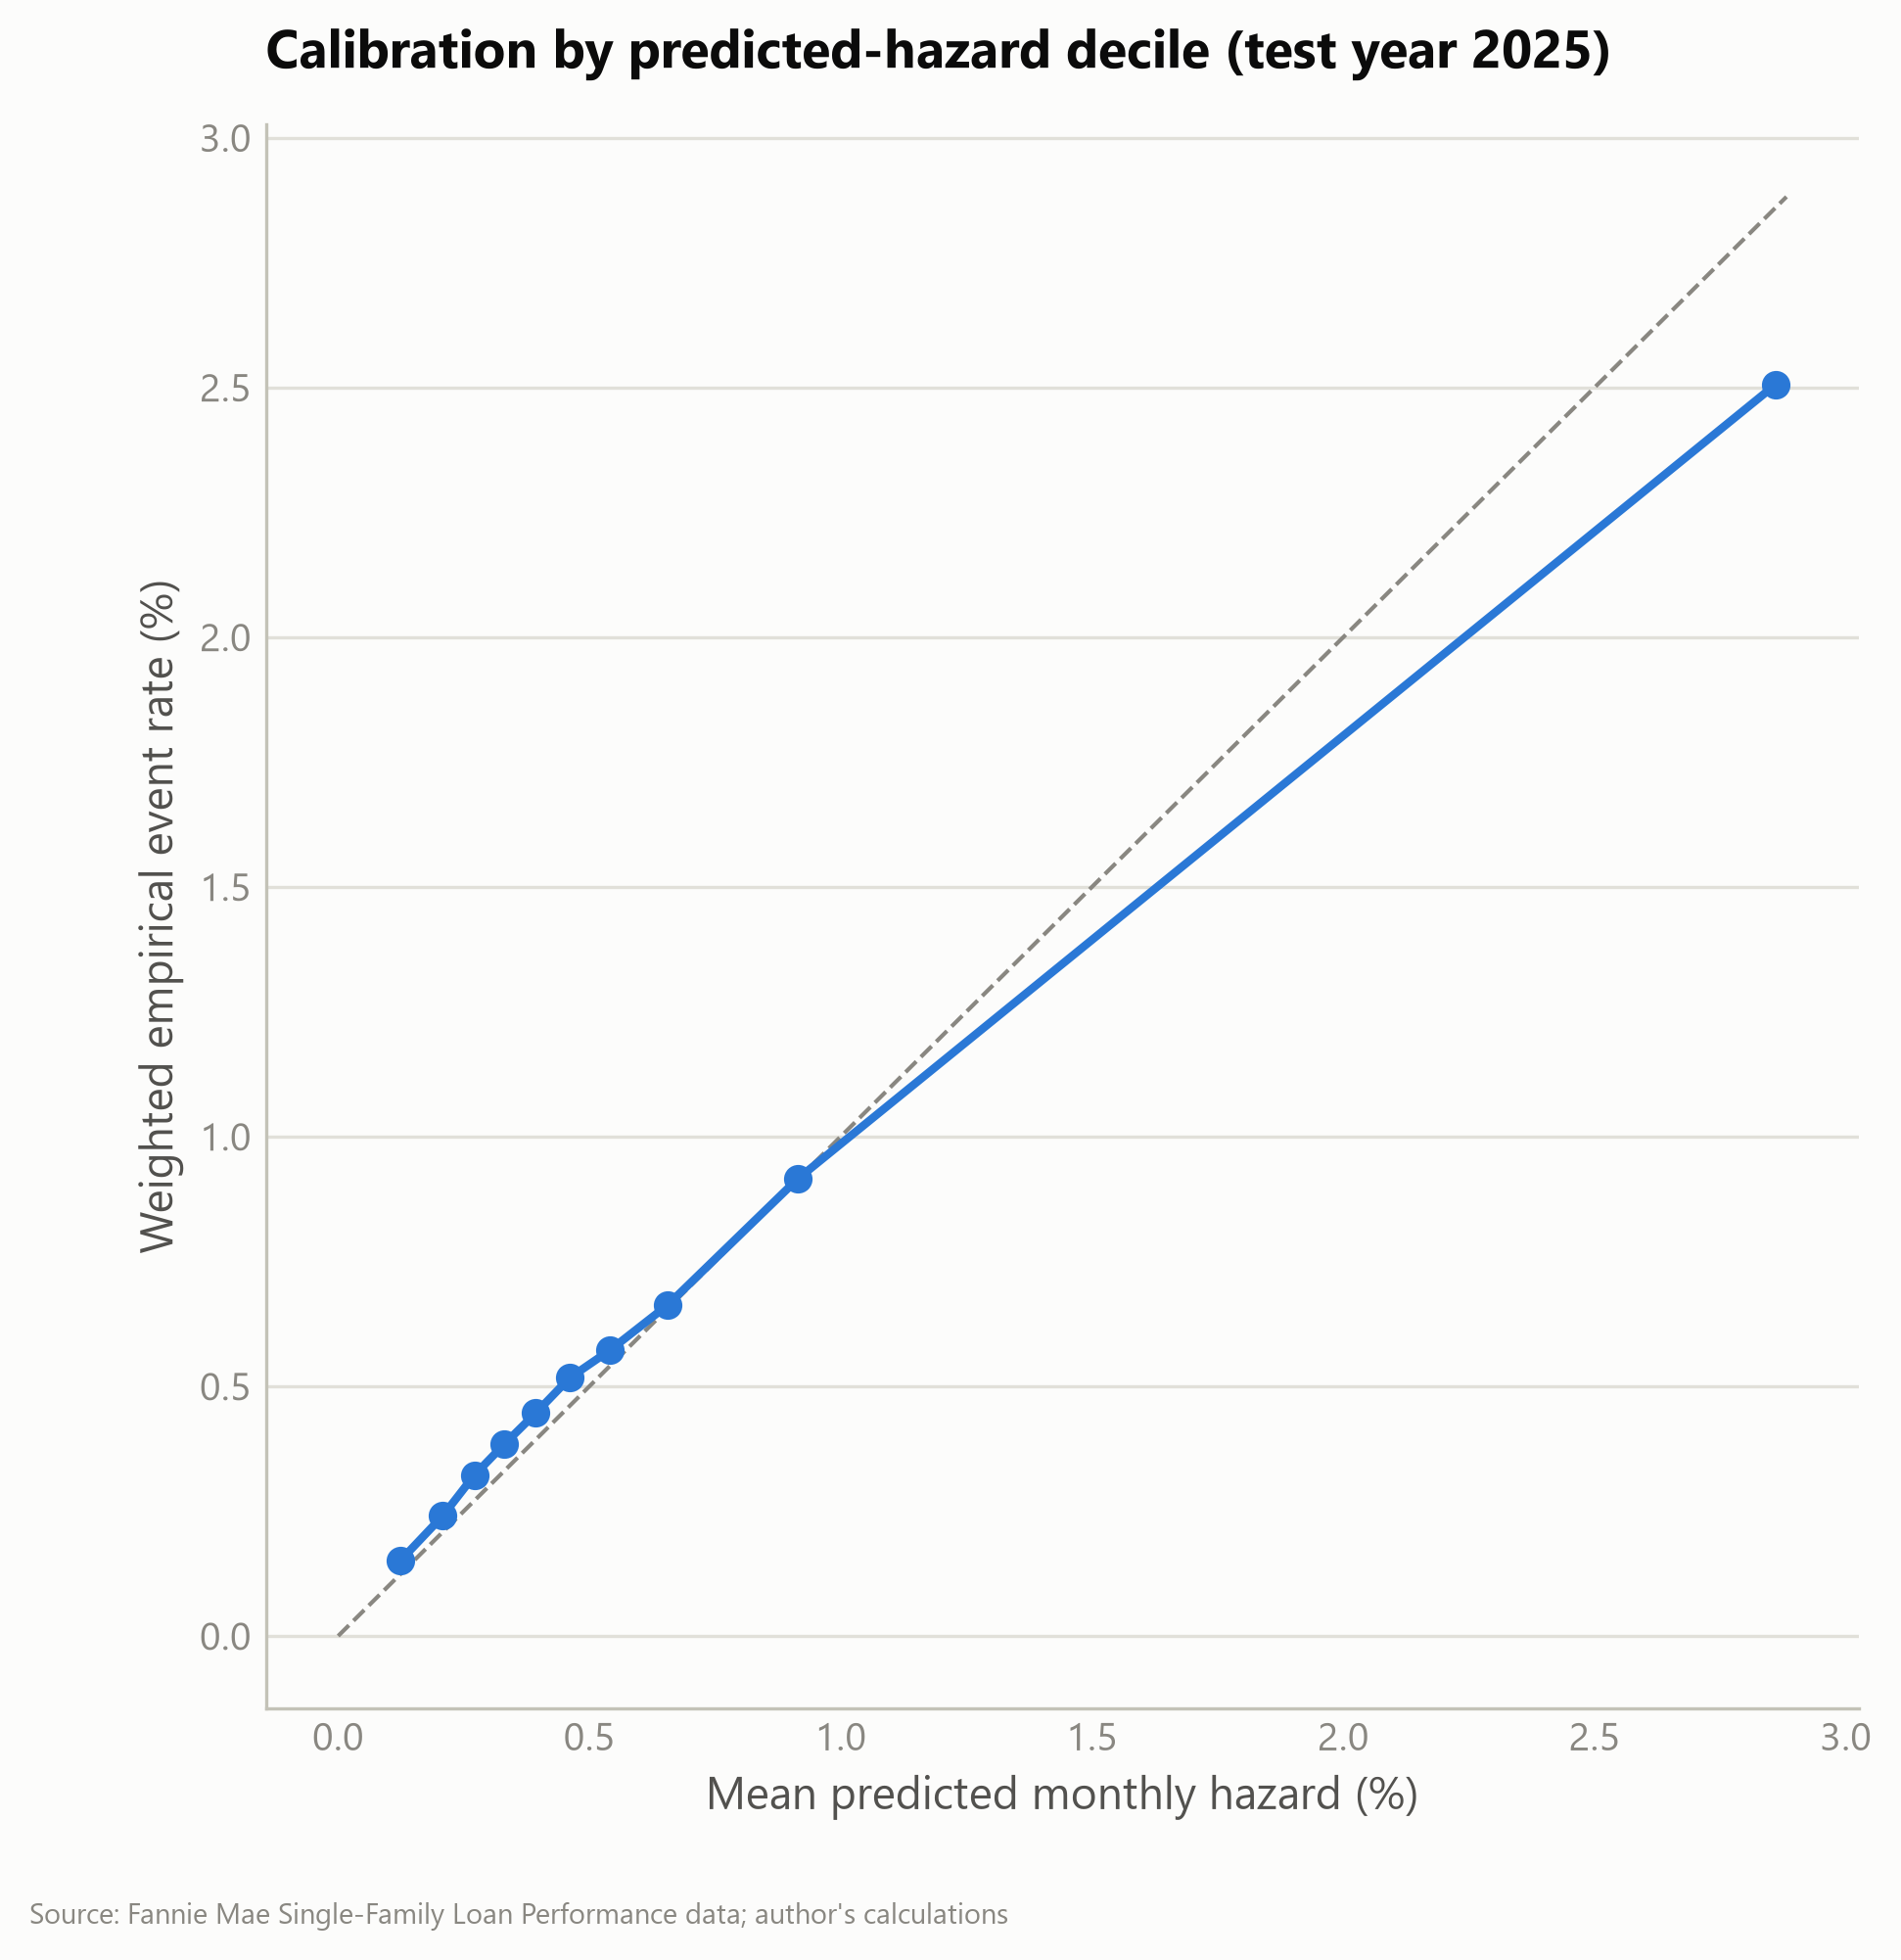
\includegraphics[width=0.6\textwidth]{figures/r1_calibration.png}
\caption{Reliability diagram on the 2025 test year: mean predicted monthly hazard versus
design-weighted empirical event rate, by predicted-hazard decile. Dashed line is the
45-degree diagonal.}
\label{fig:r1}
\end{figure}

\subsection{Cohort-level fit}

Figure~\ref{fig:r2} plots predicted against actual CPR for the 754 vintage $\times$ coupon
cohort-months (with beginning balance above \$1bn) of the 2025 test year; marker area is
proportional to cohort balance. The UPB-weighted mean absolute error is 0.86 CPR points.
Predictions track actuals closely through roughly 20 CPR, where nearly all of the balance
resides; the fastest cohort-months are modestly attenuated (predicted below actual above
approximately 25 CPR)---the cohort-level counterpart of the tail shrinkage in
Figure~\ref{fig:r1}---so point forecasts for the fastest, smallest cohorts should be read as
conservative. (The 0.86 figure equals the 0.9 entry of Table~\ref{tab:walkforward} up to the
\$1bn cohort filter and rounding.)

\begin{figure}[ht]
\centering
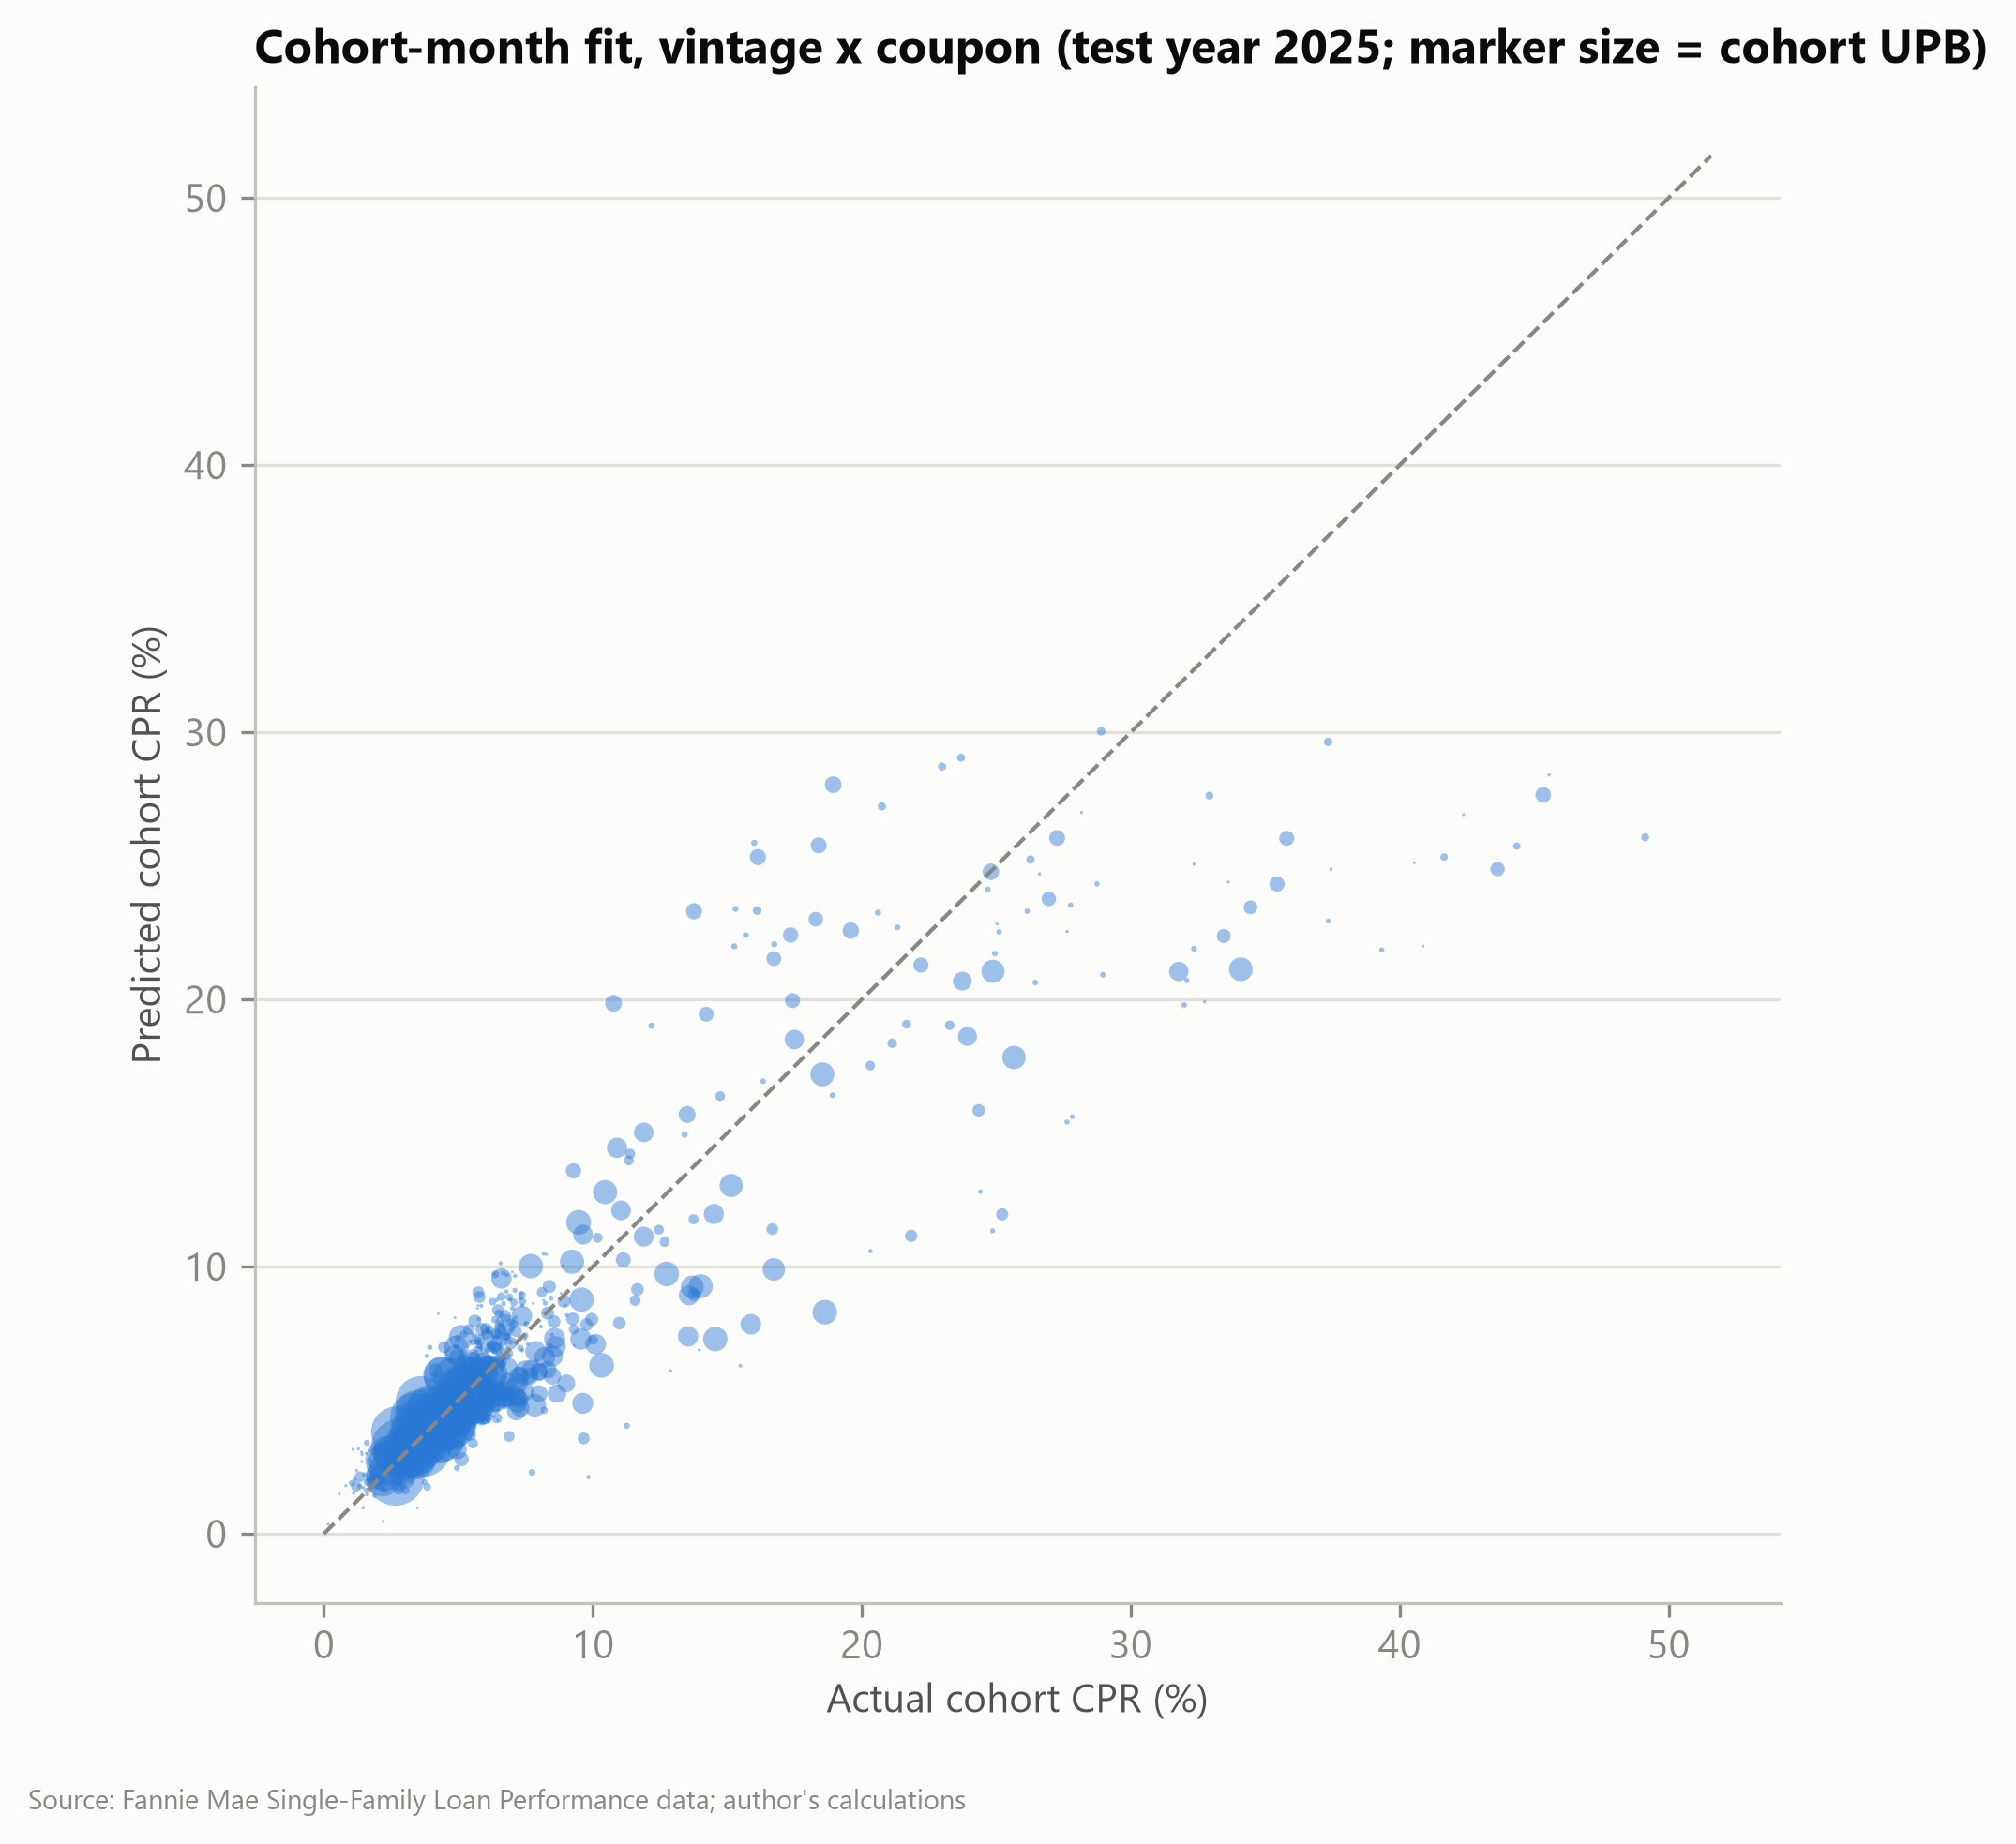
\includegraphics[width=0.6\textwidth]{figures/r2_cohort_scatter.png}
\caption{Predicted versus actual cohort CPR, 2025 test year, vintage $\times$ coupon
cohort-months with beginning UPB above \$1bn. Marker area proportional to cohort balance.}
\label{fig:r2}
\end{figure}

\subsection{Sensitivity to the non-event sampling rate}

The estimation panel retains non-event loan-months with probability $\kappa = 5\%$
(Section~\ref{sec:ipw}). Re-estimating the December 2024 model after deterministically halving
the retained non-events (an effective $\kappa$ of 2.5\%, weights doubled accordingly) leaves
results essentially unchanged (Table~\ref{tab:kappa}), consistent with the Horvitz--Thompson
argument: the downsampling rate affects efficiency, not identification.

\begin{table}[ht]
\centering
\small
\begin{tabular}{lccc}
\toprule
Panel & Training rows & AUC (2025) & Cohort CPR MAE (pts) \\
\midrule
Baseline, $\kappa = 5\%$ & 2{,}037{,}093 & 0.691 & 0.86 \\
Thinned, $\kappa = 2.5\%$ & 1{,}206{,}248 & 0.690 & 0.88 \\
\bottomrule
\end{tabular}
\caption{Sensitivity of the December 2024 model to the non-event retention rate. Evaluation on
all 2025 months.}
\label{tab:kappa}
\end{table}

\subsection{S-curve robustness across SATO buckets}

Figure~\ref{fig:r4} repeats the partial-dependence analysis of Section~\ref{sec:e2} within
tertiles of spread at origination. The regime ordering of Section~\ref{sec:e2} is preserved
within every tertile, and within every regime higher-SATO tertiles trace steeper curves ---
the composition mechanism emphasized by \citet{sancap2024scurves} --- confirming that the
S-curve rotation is not an artifact of pooling across SATO.

\begin{figure}[ht]
\centering
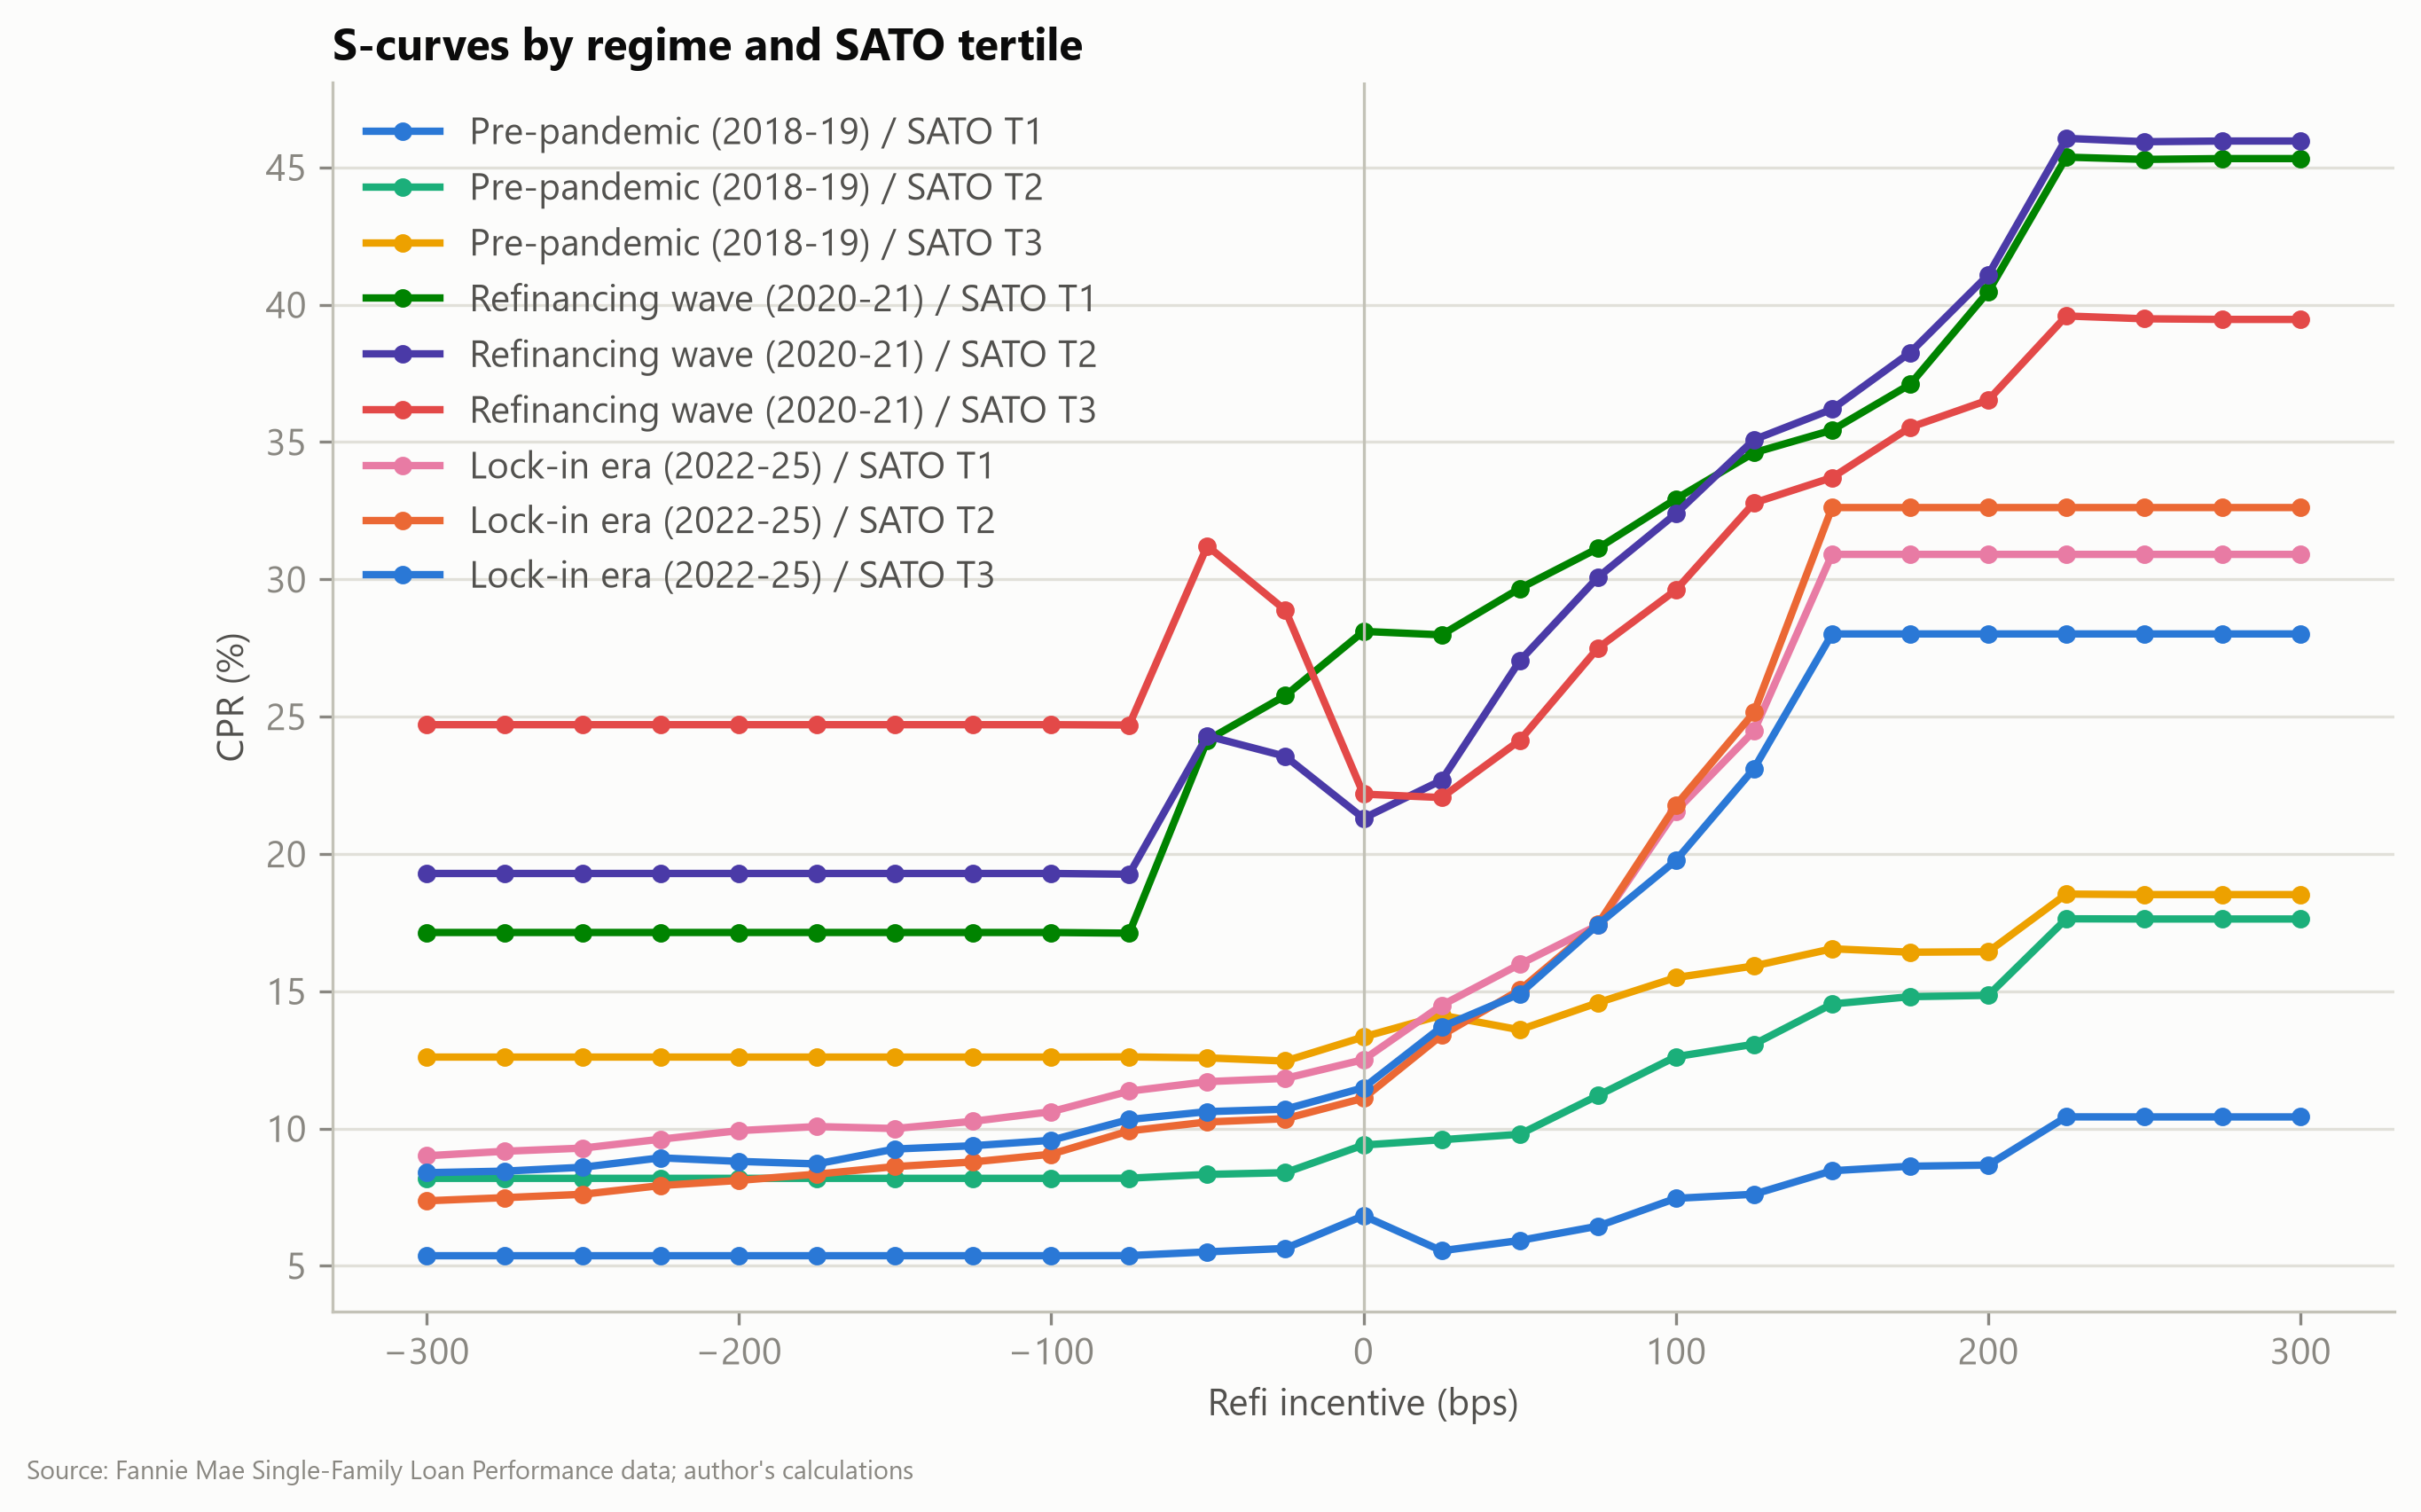
\includegraphics[width=0.9\textwidth]{figures/e2_scurves_by_sato.png}
\caption{Model-implied S-curves by regime and SATO tertile on the common reference population.}
\label{fig:r4}
\end{figure}

\end{document}
